\section{Numerical studies}
\label{sec:experiments}

The experiments compare reward allocation and reliable reporting at a fixed
physical budget. They ask how the service rule and the precision of its
reporting evidence affect regret and unresolved area. The four environments
are not the restricted family used for the two-endpoint separation result,
so they do not test its asymptotic rates.

\subsection{Protocol and competing rules}

All rewards are Bernoulli. We fix $T=20{,}000$, $\varepsilon=.30$,
$\eta=.10$, and $\delta=.05$, with eight arms by the end of each run.
There are 160 independent replications per environment. Within a replication,
each method receives the same potential reward stream for each arm: its
$n$th pull of arm $i$ reveals the same $Y_{i,n}$. The shared streams do not
force the methods to take the same actions. Arrivals precede the action,
and the report follows the observation. All methods retain previous
observations. The configuration records the arrival times, means, seeds,
and policy parameters; a policy receives current arrivals and observed
history, without future arrivals, true means, or the evaluation horizon.

The stable-benchmark environment starts with means $.65,.50$ and adds three
batches of inferior arms. The successive-improvement environment has
benchmark levels $.45,.70,.90,.98$, so a later arrival can change an
unresolved membership question. The burst environment introduces six arms
at one time, including a new best arm. In the fourth environment arrivals
stop at pull 4037, leaving nearly 16,000 pulls for recovery. Noninitial
batches arrive 36 pulls after a 100-pull admission grid; the short-period
baseline is therefore not evaluated only at its most favorable alignment.

We use two FIFO configurations of Checkpoint-UCB, denoted CP-FIFO in the
tables and CP in the figures, with service every second pull. The finer
choice $\rho=.04$ satisfies $2\rho<\eta$. Once every currently available
arm has completed its checkpoint, all $\eta$-separated arms are resolved
on the coverage event. This is not the
$\rho=\eta/4=.025$ calibration used for the worst-case area bound.
The coarser choice $\rho=.12$ retains reliable labels but does not guarantee
completeness for arbitrary environments at $\eta=.10$. Their eight-arm
quota totals are 73,083 and 8,123, respectively. In particular, the finer
configuration cannot complete all quotas within the physical budget.

Three further rules retain the coarser checkpoint report and change
allocation: CP-period8 serves the FIFO queue every eighth pull;
CP-confidence uses confidence-driven service every second pull; and
UCB-checkpoint uses full-history UCB without designated service. The
confidence-driven rule samples the widest interval among unresolved arms
and the arm with largest upper endpoint, breaking ties by sample count and
arrival order. It stops designated service when every report is resolved,
and a completed checkpoint keeps its fixed interval. These are separately
identified configurations; the FIFO guarantee is not automatically a
guarantee for every allocation variant.

Three methods combine the full-prefix confidence report with a reward or
sampling rule. UCB-prefix admits every arm immediately and uses the same
full-history UCB index as Checkpoint-UCB. Growing-MOSS uses
\[
 \hat r_i(n)+\sqrt{\frac{\max\{\log(t/(K_tn)),0\}}{n}},
\]
with infinite index at $n=0$. We do not transfer the fixed-horizon MOSS
minimax theorem to this growing-arm rule. ALL-$\varepsilon$ adaptation
uses confidence-driven service every second pull and UCB otherwise. It
retains history and can revise positive reports after arrivals. It is a
natural adaptation of confidence-based all-good-arm sampling, rather than
an implementation of FAREAST or $(\mathrm{ST})^2$.

Batch100-UCB admits waiting arms at pulls $1,101,201,\ldots$, applies UCB
to admitted reward-active arms, and retires an arm from reward sampling
when its upper bound falls below the largest active lower bound.
Observations are retained. Its report still covers every physically
arrived arm; those awaiting admission have interval $[0,1]$. Statistical
exclusion, admission, and reward retirement therefore have different
meanings in this comparison.

Table~\ref{tab:simulation} displays six methods with means and Monte Carlo
standard errors. Figure~\ref{fig:cost-area} includes all nine methods, with
error bars of 1.96 Monte Carlo standard errors. The complete allocation
table, additional paths, configuration mapping, and regret accounting are
in Appendix~\ref{app:computation}. The run records contain paired
differences, unresolved paths on the saved time grid, service pulls, and
the regret charged to service.

\input{experiments/results/table_main.tex}

\begin{figure}[t]
\centering
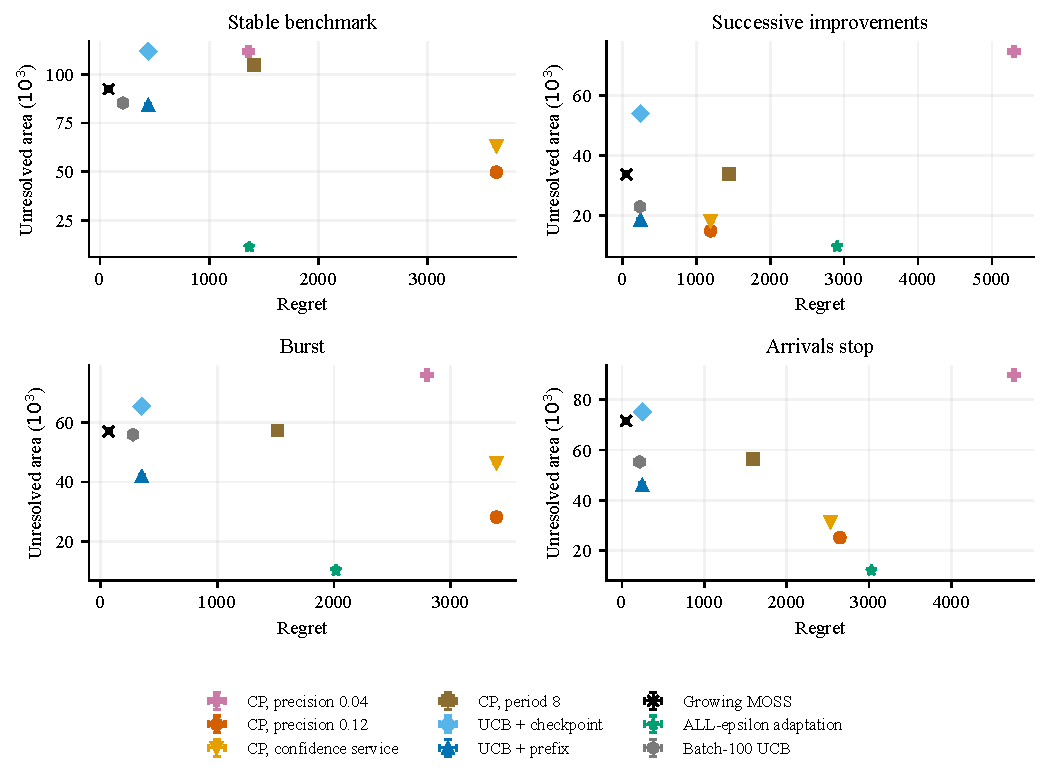
\includegraphics[width=.97\textwidth]{figures/fig_cost_area.pdf}
\caption{Regret and cumulative $\eta$-unresolved area for all nine methods.
Lower values on both axes are preferable. CP denotes the Checkpoint-UCB
configurations described in the text. Error bars quantify Monte Carlo
uncertainty. Neither checkpoint precision nor its allocation variants
uniformly dominate the confidence-based adaptation.}
\label{fig:cost-area}
\end{figure}

\subsection{Finite-budget findings and their limits}

In all 640 finer-checkpoint runs, every available arm remains unresolved
at every time step. Five to eight arms contribute to the final
$\eta$-unresolved count because the metric exempts the boundary band;
the remaining arms have not been classified. Its zero-error record
therefore does not establish useful classification at this budget.
The charged unresolved area ranges from 74,820 to 111,784. This is a
limitation of the conservative construction at the chosen budget.
The confidence-based adaptation resolves every $\eta$-separated arm by
the endpoint in all replications of these four environments.

The coarser checkpoints reduce area relative to UCB alone, but can incur
much larger regret. Under the stable benchmark, CP-FIFO has mean regret
3629.9 and area 49,718, compared with 1367.8 and 11,306 for
ALL-$\varepsilon$ adaptation. The paired differences, CP-FIFO minus the
adaptation, are $2262.1$ (standard error $11.7$) for regret and
$38{,}411.7$ (standard error $241.9$) for area. The adaptation improves
both quantities in the burst environment as well. These findings do not
support a general numerical advantage of checkpoint FIFO over a strong
history-retaining identification rule.

Under successive improvements, CP-FIFO occupies a different cost point:
regret 1194.7 and area 14,743, compared with 2905.8 and 9525 for the
adaptation. The paired regret difference is $-1711.0$ (standard error
$2.4$), and the area difference is $5217.7$ (standard error $141.1$).
This comparison does not isolate task expiration. The adaptation uses
all 10,000 designated service pulls, whereas coarse CP uses about 5,786;
some remaining questions fall inside the unpenalized boundary band.
The regret difference can therefore partly reflect different stopping
rules for reporting work. Identifying the mechanism requires a comparison
with the same boundary tolerance and service requirement. These observed
cost points do not estimate an optimal frontier.

Growing-MOSS has the smallest mean regret in all four environments,
between 52.0 and 77.3, while leaving substantially larger unresolved
areas. Small regret alone provides little evidence of timely set
maintenance; it does not rule out adding an effective certification
layer to that allocation rule. Explicit service pays for observations of
inferior arms. Reducing service from every second to every eighth pull
generally reduces regret and enlarges unresolved area. Confidence-driven
checkpoint service does not uniformly improve either criterion.

\begin{figure}[t]
\centering
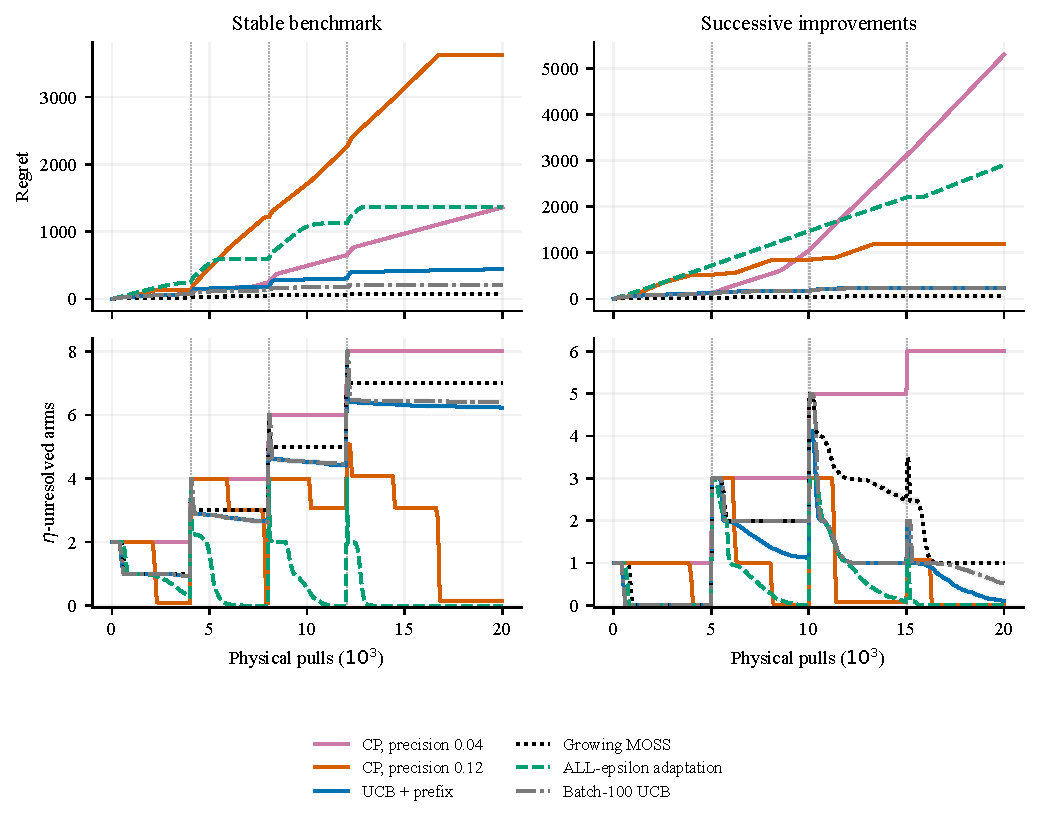
\includegraphics[width=.98\textwidth]{figures/fig_paths_pair1.pdf}
\caption{Mean regret and mean $\eta$-unresolved arm counts at the physical
sampling clock. Bands are 1.96 Monte Carlo standard errors; vertical dotted
lines mark arrivals. Stable and improving benchmarks are shown here,
with the other two environments in Appendix~\ref{app:computation}.
The six main-table methods are displayed. The saved results retain all
nine methods and their paths on the common observation grid.}
\label{fig:paths}
\end{figure}

For Batch100-UCB, the admission-delay contributions to regret are $0$,
$33.92$, $16.00$, and $22.40$ in the four environments. No historical
retirement deficit occurred in these runs. Appendix~\ref{app:computation}
defines this decomposition and distinguishes it from learning within the
reward-active set.

There were no incorrect positive or negative reports in any of the 5,760
runs. For one fixed method and environment, zero failures in 160
replications gives an exact one-sided 95\% upper confidence bound below
0.0186 on its failure probability. This finite experiment does not
establish uniform reliability over all environments and times. Nor do
the eight-arm comparisons validate the asymptotic lower bounds, settle
the critical logarithmic gap, or establish checkpoint optimality.
They quantify the finite-budget cost of the conservative quotas and
show why reward and maintenance must be reported together.

